\documentclass[11pt,a4paper]{article}

\usepackage[margin=2cm,top=2.2cm,bottom=2.2cm]{geometry}
\usepackage{graphicx}
\usepackage{adjustbox}
\usepackage{titlesec}
\usepackage{enumitem}
\usepackage{hyperref}
\usepackage{fancyhdr}
\usepackage{xcolor}
\usepackage{setspace}
\usepackage{helvet}
\usepackage[T1]{fontenc}
\usepackage{tikz}
\usepackage{float}
\usepackage{placeins}
\usepackage{pdflscape}
\usepackage{caption}

\setlength{\parskip}{0.45em plus 0.1em minus 0.05em}
\setlength{\parindent}{0pt}
\captionsetup{font=small, labelfont=bf, skip=6pt}
\floatplacement{figure}{htbp}

\renewcommand{\familydefault}{\sfdefault}

\definecolor{brandblue}{HTML}{0c3472}
\definecolor{brandlight}{HTML}{c8d7eb}
\definecolor{textgray}{HTML}{475569}

\hypersetup{
    colorlinks=true,
    linkcolor=brandblue,
    urlcolor=brandblue,
    pdftitle={Revenue Navigator AI Framework},
    pdfauthor={Revenue Navigator}
}

\pagestyle{fancy}
\fancyhf{}
\fancyhead[L]{\small\textcolor{textgray}{Revenue Navigator --- Customer Success}}
\fancyhead[R]{\small\textcolor{textgray}{Predictive Revenue Platform}}
\fancyfoot[C]{\small\textcolor{textgray}{\thepage}}
\renewcommand{\headrulewidth}{0.4pt}
\renewcommand{\footrulewidth}{0pt}

\titleformat{\section}{\Large\bfseries\color{brandblue}}{}{0em}{}[\titlerule]
\titleformat{\subsection}{\large\bfseries\color{brandblue}}{}{0em}{}
\titlespacing*{\section}{0pt}{1em}{0.5em}
\titlespacing*{\subsection}{0pt}{0.8em}{0.35em}

\newcommand{\capblock}[3]{%
    \vspace{0.25em}
    \noindent\textbf{#1}\\[0.15em]
    #2
    \vspace{0.2em}
    \noindent\textit{Business value:} #3
    \vspace{0.35em}
}

\newcommand{\docfig}[5]{%
    \begin{figure}[#1]
        \centering
        \adjustbox{max width=\textwidth, max height=#2, center}{%
            \includegraphics{#3}%
        }%
        \caption{#4}
        \label{#5}
    \end{figure}%
}

\newcommand{\makecover}{%
    \thispagestyle{empty}
    \begin{center}
        \vspace*{1.5cm}
        {\color{brandblue}\rule{\textwidth}{2pt}}\\[0.8cm]
        {\fontsize{28}{34}\selectfont\bfseries\color{brandblue} Revenue Navigator}\\[0.3cm]
        {\large Predictive Customer Success Platform}\\[1.2cm]
        {\fontsize{22}{28}\selectfont\bfseries AI-Powered Renewal}\\[0.2cm]
        {\fontsize{22}{28}\selectfont\bfseries \& Upsell Operations Framework}\\[1.5cm]
        {\large B2B Predictive Customer Success Platform}\\[2cm]
        
\begin{tikzpicture}
            \fill[brandlight, rounded corners=4pt] (0,0) rectangle (10,1.2);
            \node at (5,0.6) {\textbf{\color{brandblue} Confidential --- For Management Review}};
        \end{tikzpicture}\\[2cm]
        {\large \today}\\[0.5cm]
        {\color{textgray} Platform Architecture \& Vision Document}
        \vfill
        {\color{brandblue}\rule{\textwidth}{2pt}}
    \end{center}
    \newpage
}

\begin{document}

\makecover

\tableofcontents
\newpage

% =============================================================================
\section{Executive Summary}

\textbf{Revenue Navigator} is a predictive customer success and revenue operations platform that helps CSM and RevOps teams stay ahead of churn, automate renewal outreach, and discover upsell opportunities across the entire client portfolio.

This document describes the \textbf{AI-powered renewal and upsell operations framework} that unifies account intelligence, multi-channel outreach, and predictive scoring into a single revenue command center.

\textbf{What leadership and CSM teams will gain:}
\begin{itemize}[leftmargin=1.5em, itemsep=0.3em]
    \item Predictive \textbf{churn risk} and \textbf{account health scoring} before renewals are at risk
    \item Automated \textbf{AI voice}, \textbf{email drip campaigns}, and \textbf{WhatsApp outreach} at lifecycle milestones
    \item Intelligent \textbf{upsell opportunity discovery} and expansion revenue tracking
    \item Real-time \textbf{pipeline, MRR, and sentiment analytics} for executive decision-making
    \item An \textbf{LLM-powered assistant} and \textbf{ML scoring engine} for natural-language queries and forward-looking predictions
\end{itemize}

The framework enables organisations to operate as proactive, data-driven customer success teams --- reducing reactive firefighting and maximising retention and expansion revenue.

% =============================================================================
\section{About Revenue Navigator}

\textbf{Revenue Navigator} is an enterprise-grade predictive customer success platform, designed for B2B organisations managing complex renewal cycles, multi-stakeholder accounts, and expansion opportunities.

The platform acts as a \textbf{24/7 AI co-pilot} for Revenue Operations and Customer Success departments, combining:
\begin{itemize}[leftmargin=1.5em, itemsep=0.2em]
    \item Predictive analytics on account health, churn, and renewal probability
    \item Intelligent automation across voice, email, and messaging channels
    \item A unified view of pipeline health, MRR, and campaign performance
\end{itemize}

% =============================================================================
\section{Business Challenge}

In competitive B2B environments, customer success teams face persistent operational gaps:

\begin{itemize}[leftmargin=1.5em, itemsep=0.3em]
    \item \textbf{Reactive churn management} --- teams learn about at-risk accounts only when customers complain or contracts lapse
    \item \textbf{Manual outreach overload} --- CSMs spend hours on routine renewal calls, follow-up emails, and status checks
    \item \textbf{Fragmented customer data} --- usage metrics, support tickets, CRM records, and communication history live in separate systems
    \item \textbf{Missed expansion revenue} --- upsell signals in usage patterns and sentiment go undetected until competitors intervene
    \item \textbf{Inconsistent renewal execution} --- no standardised lifecycle playbook across accounts of different health and maturity
\end{itemize}

Without unified intelligence, leadership lacks early warning on revenue at risk and CSMs cannot prioritise the accounts that need intervention most.

% =============================================================================
\section{Proposed Solution Overview}

The proposed \textbf{AI-Powered Renewal \& Upsell Operations Ecosystem} provides centralized, predictive visibility into every account --- from onboarding through renewal, adoption, and expansion.

The system integrates data from CRM, billing, support, and communication channels to create a \textbf{unified revenue operations dashboard}. An AI decision engine continuously scores accounts, predicts churn, recommends next-best actions, and triggers automated outreach --- while CSMs retain oversight through escalation workflows for high-risk accounts.

The following sections present the architecture (Figure~\ref{fig:architecture}), platform technology stack (Figure~\ref{fig:platform}), lifecycle classification (Figure~\ref{fig:lifecycle}), account journey (Figure~\ref{fig:journey}), revenue ecosystem (Figure~\ref{fig:ecosystem}), and detailed module flows (Figures~\ref{fig:flow-scoring}--\ref{fig:flow-analytics}).

% =============================================================================
\section{Architecture Overview}

The architecture flows through eight interconnected stages, from data input to measurable business outcomes:

\begin{enumerate}[leftmargin=1.5em, itemsep=0.4em]
    \item \textbf{Input Sources} --- CRM, usage metrics, support tickets, email replies, call transcripts, contracts, payments, webhooks
    \item \textbf{Data Unification} --- Central collection, account matching, LLM sentiment extraction, validation, real-time sync
    \item \textbf{AI Decision Engine} --- ML scoring (churn, health, upsell, renewal), LLM sentiment, NBA recommendations, model orchestration
    \item \textbf{Management Review} --- Straight-through outreach for low-risk accounts; CSM escalation for critical churn and SLA breaches
    \item \textbf{Core Renewal \& Upsell Workflow} --- Pipeline management, quotes, email/voice/WhatsApp outreach, contract renewal
    \item \textbf{Enterprise Integration} --- Salesforce, Stripe, Twilio, email providers, API gateway, webhooks
    \item \textbf{Analytics \& Governance} --- KPI dashboards, campaign ROI, model monitoring, RBAC, audit trail
    \item \textbf{Business Outcomes} --- Reduced churn, faster renewals, expansion revenue, lower ops cost, higher CSM productivity
\end{enumerate}

A secure data foundation supports the entire platform, with a continuous feedback loop that refines scoring models through performance feedback and new account data.

\begin{landscape}
\thispagestyle{fancy}
\begin{figure}[p]
    \vspace*{-0.8cm}
    \centering
    \adjustbox{max width=\linewidth, max height=0.76\paperheight, center}{%
        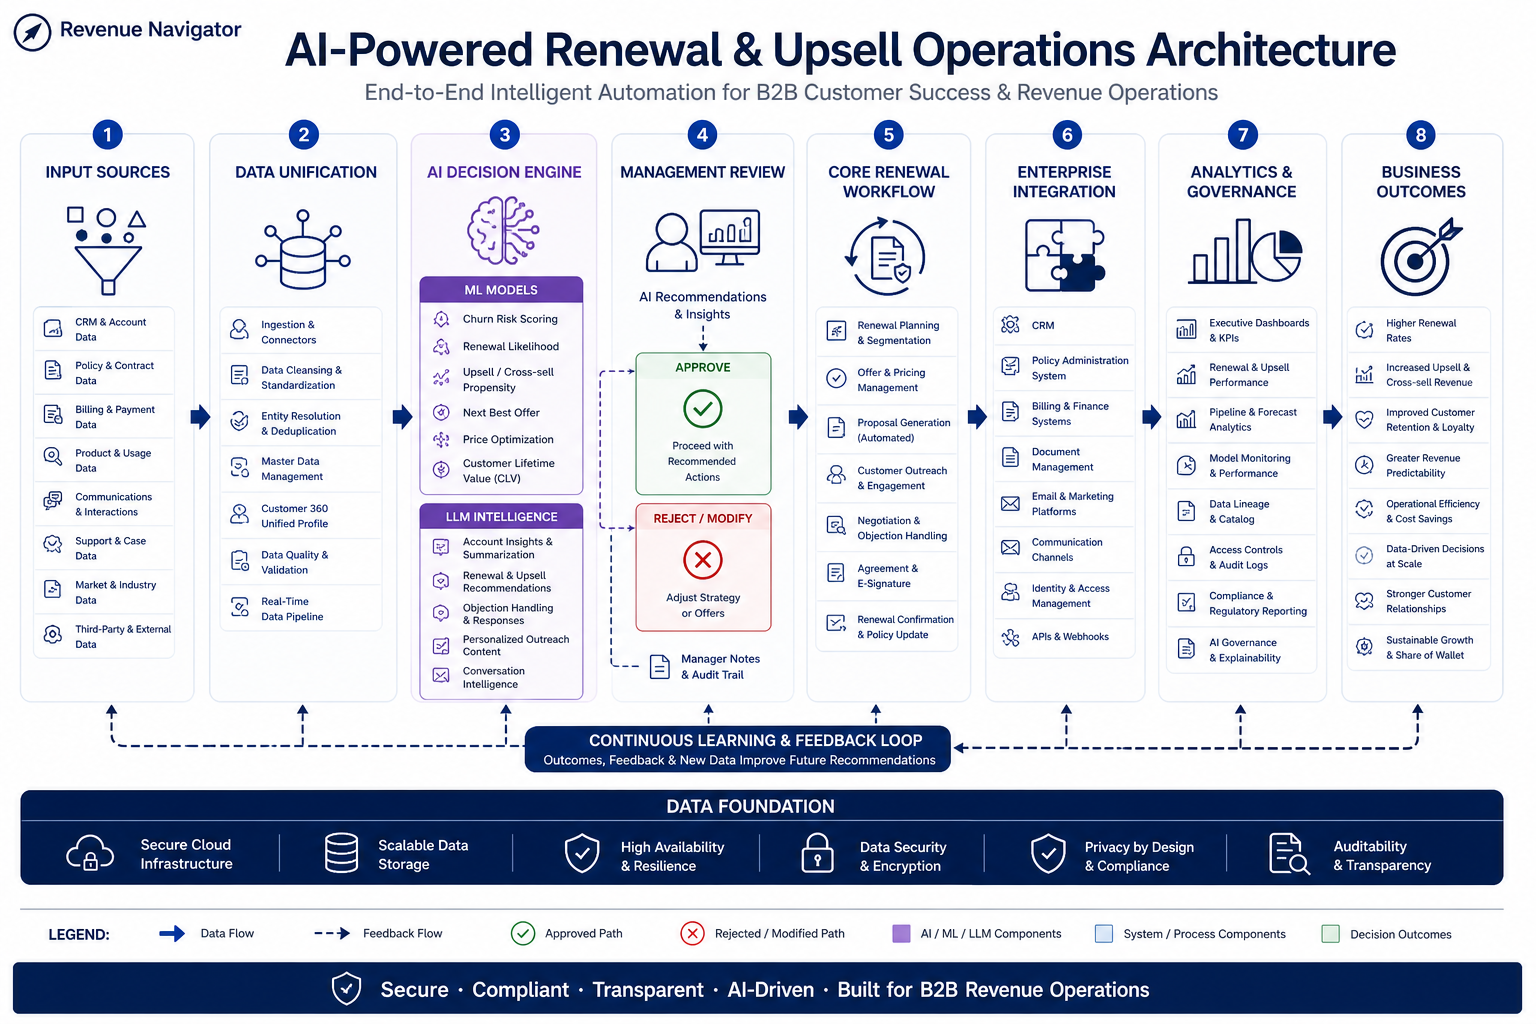
\includegraphics{images/rnu-architecture-flow.png}%
    }
    \caption{AI-Powered Renewal \& Upsell Operations Architecture --- end-to-end intelligent automation for B2B customer success and revenue operations.}
    \label{fig:architecture}
    \vspace*{-0.4cm}
\end{figure}
\end{landscape}

\FloatBarrier
% =============================================================================
\section{Platform \& AI Technology}

Beyond business dashboards, Revenue Navigator includes a focused AI and technology stack designed for enterprise B2B scale (Figure~\ref{fig:platform}).

\docfig{htbp}{0.46\textheight}{images/rnu-platform-architecture.png}{Revenue Navigator platform architecture --- technology layers from presentation to data foundation.}{fig:platform}

\subsection{ML Scoring Engine}

Predictive scoring models analyse account behaviour, usage, sentiment, and engagement to generate actionable intelligence:
\begin{itemize}[leftmargin=1.5em, itemsep=0.25em]
    \item \textbf{Health Score (0--100)} --- composite of utilization (40\%), sentiment (30\%), and recency (30\%)
    \item \textbf{Churn Probability (0.0--1.0)} --- inverse of health with urgency penalty for near-term renewals
    \item \textbf{Relationship Score} --- CSM engagement quality from contact recency and sentiment
    \item \textbf{Renewal Score} --- likelihood and timing of successful contract renewal
    \item \textbf{Upsell Detection} --- heuristics on health, utilization, and company size for expansion signals
\end{itemize}

Scores are orchestrated by a \textbf{unified predictor pipeline}, pushed to Supabase on schedule, and triggerable on demand via the ML API.

\subsection{LLM AI Assistant \& Sentiment}

\textbf{Azure OpenAI} (GPT-4o via LangChain) powers:
\begin{itemize}[leftmargin=1.5em, itemsep=0.25em]
    \item \textbf{Sentiment analysis} --- JSON-structured sentiment scoring on customer communications
    \item \textbf{Email personalization} --- LLM-generated outreach content tailored to account context
    \item \textbf{Voice bot conversations} --- browser-based and outbound call dialogue with Azure Speech STT/TTS
    \item \textbf{Call summaries} --- automated post-call intelligence for CSM review
\end{itemize}

\subsection{Lifecycle Engine \& Next Best Action}

The \textbf{lifecycle engine} classifies every account into stages --- Protect, Renew, Adopt, Expand, Activate --- and generates \textbf{Next Best Action (NBA)} recommendations including channel (call, email, WhatsApp), due date, and specific action templates.

\subsection{Multi-Channel Outreach Layer}

\begin{itemize}[leftmargin=1.5em, itemsep=0.25em]
    \item \textbf{AI Voice Agent} --- Twilio outbound calls with Azure OpenAI conversation handling
    \item \textbf{Email campaigns} --- Resend, SendGrid, or SMTP with drip scheduling and LLM personalization
    \item \textbf{WhatsApp messaging} --- Twilio WhatsApp for adoption check-ins and quick engagement
    \item \textbf{Manual triggers} --- CSM-initiated outreach from the operations console
\end{itemize}

\subsection{Integration \& Data Foundation}

\begin{itemize}[leftmargin=1.5em, itemsep=0.25em]
    \item \textbf{FastAPI REST gateway} --- secure API for frontend, webhooks, and partner integrations
    \item \textbf{Salesforce \& Stripe connectors} --- CRM sync and billing data integration
    \item \textbf{JWT authentication} --- role-based secure access for CSM and admin users
    \item \textbf{Supabase operational store} --- primary data layer with SQLite/PostgreSQL fallback
    \item \textbf{Scheduled jobs} --- automated ML pipeline runs, campaign execution, and email polling
\end{itemize}

% =============================================================================
\section{Customer Lifecycle Classification}

Unlike a simple linear pipeline, Revenue Navigator uses a \textbf{priority-based classification model}. Each account is evaluated daily and assigned to \textbf{one primary lifecycle stage} based on the highest-priority matching signal (Figure~\ref{fig:lifecycle}).

\begin{itemize}[leftmargin=1.5em, itemsep=0.3em]
    \item \textbf{Protect} (Priority 1, Call) --- At-risk or critical health; executive escalation and P1 support sync; due today
    \item \textbf{Renew} (Priority 2, Email) --- Renewal within 90 days; early proposal and QBR scheduling; due this week
    \item \textbf{Adopt} (Priority 3, WhatsApp) --- Low utilization or deployment gaps; partner check-in; due within 5 days
    \item \textbf{Expand} (Priority 4, Email) --- High health with growth signals; expansion package and upsell quote; due this week
    \item \textbf{Activate} (Priority 5, Call) --- New account onboarding; kickoff workshop and CSM assignment; due within 3 days
\end{itemize}

The lifecycle engine routes each account to the correct stage, generates a Next Best Action, and triggers the recommended outreach channel.

\docfig{htbp}{0.48\textheight}{images/rnu-lifecycle-flow.png}{Lifecycle classification flow --- accounts are routed to one primary stage by priority, not a linear sequence.}{fig:lifecycle}

\subsection{End-to-End Account Journey}

Figure~\ref{fig:journey} shows the realistic B2B revenue journey: new accounts enter through \textbf{Activate}, progress through \textbf{Adopt}, then enter continuous monitoring where the scoring engine routes accounts to Protect, Renew, or Expand based on live signals.

\docfig{htbp}{0.42\textheight}{images/rnu-account-journey.png}{End-to-end account revenue journey from onboarding through renewal with continuous monitoring loop.}{fig:journey}

\FloatBarrier
% =============================================================================
\section{Revenue Operations Ecosystem}

The Revenue Operations Center serves as the intelligence hub, connecting customer accounts, CSM teams, outreach channels, and enterprise integrations into a single actionable view (Figure~\ref{fig:ecosystem}).

\docfig{htbp}{0.52\textheight}{images/rnu-ecosystem-map.png}{B2B revenue operations ecosystem --- the Revenue Operations Center connects accounts, CSMs, channels, and integrations.}{fig:ecosystem}

% =============================================================================
\section{Capability Modules}

The framework comprises six integrated capability modules. Each module answers specific management questions and drives measurable revenue outcomes.

\subsection{Predictive Pipeline \& Account Scoring}

\capblock{Purpose}{%
Gain complete visibility into the customer portfolio. ML scoring models generate Account Health Scores, Churn Risk predictions, and Relationship Scores instantly. Track accounts through customised renewal stages and prioritise intervention by risk level.}{%
Identify at-risk accounts before churn occurs, focus CSM time on highest-impact accounts, and maintain a healthy renewal pipeline with data-driven prioritisation.}

\docfig{htbp}{0.28\textheight}{images/rnu-flow-scoring.png}{Predictive pipeline and account scoring flow --- from data ingestion to CSM action queue.}{fig:flow-scoring}

\subsection{AI Voice Renewal Agent}

\capblock{Purpose}{%
Automate routine renewal follow-ups with intelligent AI voice agents. Configure outbound calls at critical quarterly milestones (Q3 check-ins, Q4 renewals), handle common objections, and escalate complex negotiations to human CSMs seamlessly.}{%
Reduce manual call volume, ensure consistent renewal touchpoints across all accounts, and free CSMs to focus on strategic high-value relationships.}

\docfig{htbp}{0.28\textheight}{images/rnu-flow-voice.png}{AI voice renewal agent flow --- outbound call, live AI dialogue, and CSM escalation path.}{fig:flow-voice}

\subsection{Automated Campaign Manager}

\capblock{Purpose}{%
Design and execute email drip campaigns tailored to customer segments. Automated reminders and promotional workflows guide accounts from ``At Risk'' back to ``Healthy'' with LLM-personalized content.}{%
Maximise customer engagement with minimal manual effort, improve renewal conversion rates, and maintain consistent communication cadence.}

\docfig{htbp}{0.28\textheight}{images/rnu-flow-campaign.png}{Automated email campaign manager flow --- segmentation, LLM personalization, send, track, and re-score.}{fig:flow-campaign}

\subsection{Upsell Opportunity Discovery}

\capblock{Purpose}{%
Detect expansion signals from usage patterns, health scores, and company profiles. Surface upsell opportunities with product recommendations and estimated expansion value in the opportunities dashboard.}{%
Capture expansion revenue that would otherwise be missed, align product recommendations with account readiness, and grow net revenue retention.}

\docfig{htbp}{0.28\textheight}{images/rnu-flow-upsell.png}{Upsell opportunity discovery flow --- signal detection through pipeline to revenue forecast.}{fig:flow-upsell}

\subsection{Lifecycle Engine \& Next Best Action}

\capblock{Purpose}{%
Automatically classify accounts into lifecycle stages (Protect, Renew, Adopt, Expand, Activate) and generate daily NBA recommendations with channel, action, and due date for each account.}{%
Eliminate guesswork in CSM daily planning, ensure the right action reaches the right account at the right time, and standardise best-practice playbooks across the team.}

\docfig{htbp}{0.28\textheight}{images/rnu-flow-nba.png}{Lifecycle engine and next-best-action flow --- daily scan, stage match, outreach execution.}{fig:flow-nba}

\subsection{Analytics \& Revenue Intelligence}

\capblock{Purpose}{%
Live dashboards for MRR, expansion revenue, churn rate, and portfolio health. Advanced analytics with revenue trend lines, risk distribution charts, campaign ROI tracking, and sentiment trends.}{%
Enable executive-level revenue visibility, measure outreach effectiveness, and support board-level reporting with real-time data.}

\docfig{htbp}{0.28\textheight}{images/rnu-flow-analytics.png}{Analytics and revenue intelligence flow --- data aggregation to executive dashboards and MIS exports.}{fig:flow-analytics}

% =============================================================================
\section{Strategic Benefits}

The proposed AI-powered revenue ecosystem will significantly enhance customer success efficiency and revenue visibility:

\begin{itemize}[leftmargin=1.5em, itemsep=0.35em]
    \item \textbf{Proactive churn prevention} through predictive scoring before contracts are at risk
    \item \textbf{Automated multi-channel outreach} reducing manual CSM workload by up to 60\%
    \item \textbf{Expansion revenue growth} through intelligent upsell discovery
    \item \textbf{Unified revenue intelligence} across pipeline, sentiment, and campaign performance
    \item \textbf{Standardised lifecycle playbooks} ensuring consistent execution across all accounts
    \item \textbf{Faster renewal cycles} through timely, personalised outreach at every milestone
    \item \textbf{Executive dashboards} for real-time MRR, churn, and health visibility
    \item \textbf{AI-augmented CSM productivity} with LLM assistant and automated recommendations
    \item \textbf{Enterprise-grade integrations} with Salesforce, Stripe, and communication platforms
    \item \textbf{Continuous model improvement} through feedback loops and performance monitoring
\end{itemize}

% =============================================================================
\section{Conclusion}

The proposed \textbf{AI-Powered Renewal \& Upsell Operations Framework} will transform how organisations manage customer success and revenue operations.

By integrating predictive scoring, multi-channel AI agents, lifecycle intelligence, and real-time analytics into a single platform, teams can achieve higher retention rates, faster renewals, greater expansion revenue, and superior CSM productivity.

This framework positions adopters as technologically advanced, proactively intelligent B2B customer success organisations.

\vspace{1.5em}
\begin{center}
    {\color{brandblue}\rule{0.6\textwidth}{1.5pt}}\\[0.5em]
    \textit{Secure \textperiodcentered\ Compliant \textperiodcentered\ Transparent \textperiodcentered\ AI-Driven}\\[0.3em]
    \textbf{\color{brandblue}Built for B2B Revenue Operations}
\end{center}

\end{document}
